\documentclass[11pt]{article}

\usepackage[margin=1in]{geometry}
\usepackage{amsmath, amssymb}
\usepackage{graphicx}
\usepackage{listings}
\usepackage{xcolor}
\usepackage{caption}
\usepackage{booktabs}
\usepackage{siunitx}
\usepackage{microtype}
\usepackage{url}
\usepackage{hyperref}

\hypersetup{
  colorlinks=true,
  linkcolor=blue!50!black,
  urlcolor=blue!50!black,
  citecolor=blue!50!black
}

\lstdefinestyle{mystyle}{
  basicstyle=\ttfamily\footnotesize,
  columns=fullflexible,
  keywordstyle=\color{blue!70!black}\bfseries,
  commentstyle=\color{gray!70!black}\itshape,
  stringstyle=\color{green!60!black},
  showstringspaces=false,
  breaklines=true,
  breakatwhitespace=true,
  frame=single,
  rulecolor=\color{gray!40},
  numbers=left,
  numberstyle=\tiny\color{gray!60},
  numbersep=6pt,
  xleftmargin=2.2em,
  framexleftmargin=1.8em,
  aboveskip=8pt,
  belowskip=8pt
}
\lstset{style=mystyle}

\title{\vspace{-2.5em}GPU-Accelerated Wilson--Cowan Neural Field\\ Simulation with cuFFT}

\author{Will Suan \\
  EID: whs726 \quad TACC: wsuan \\
  \url{william.suan@protonmail.com}}

\date{COE 379 Final Project --- Spring 2026 \\ TACC Frontera}

\begin{document}
\maketitle

\begin{abstract}
  \noindent The Wilson--Cowan equations are a mean-field model of coupled
  excitatory and inhibitory neural populations on a 2D cortical sheet.
  Under a Mexican-hat coupling profile, the model spontaneously produces
  the geometric hallucination patterns --- spirals, tunnels, lattices ---
  derived by Ermentrout and Cowan in 1979. This project implements the
  equations on a periodic 2D grid with FFT-based spatial coupling via
  NVIDIA cuFFT and forward Euler time integration, running on the
  Quadro RTX 5000 GPUs of a Frontera \texttt{rtx-dev} node. I measure
  per-step cost and throughput across grid sizes from $128^2$ to $4096^2$,
  compare the measured scaling to the theoretical $O(N^{2} \log N)$ cost
  of the FFT-based kernel, and report near-linear speedup of an
  embarrassingly parallel 4-GPU parameter sweep. A \SI{10}{\second}
  video of the ``spirals'' regime is attached to the repository
  (\url{https://github.com/willsuan/neural-field-gpu}).
\end{abstract}

% --------------------------------------------------------------------
\section{Introduction}
\label{sec:intro}

The Wilson--Cowan equations~\cite{wilson1972} describe the mean firing
rates of two interacting neural populations, excitatory ($E$) and
inhibitory ($I$), distributed over a continuous 2D cortical sheet. Under
the right combination of couplings the homogeneous steady state becomes
unstable to spatial perturbations, and the system organizes into
stationary stripes and spots, rotating spiral waves, or traveling
plane waves~\cite{ermentrout1979,bressloff2001}. The resulting pattern
basis reproduces the ``form constants'' reported in the perceptual
literature on drug-induced hallucinations and migraine aura --- which
gives an otherwise abstract PDE system an unusually concrete payoff.

Computationally, the interesting feature of the model is that the
spatial coupling is \emph{non-local}: each cell interacts with every
other cell through a Gaussian kernel $K(\mathbf{r})$. A naive
cell-by-cell evaluation costs $O(N^{2} K^{2})$ per time step, where $N$
is the grid side and $K$ is the kernel radius in cells. At realistic
radii ($K \!\sim\! 10$--$30$) and grid sizes ($N \!\geq\! 1024$), this
is prohibitive. FFT-based convolution --- transforming the problem to
Fourier space, multiplying, and transforming back --- reduces the cost
to $O(N^{2} \log N)$ per step, which is roughly four orders of
magnitude cheaper at $N = 1024$. The GPU is an attractive target because
both the FFTs (dense, regular, memory-bandwidth-heavy) and the
pointwise Wilson--Cowan update (embarrassingly parallel, trivially
vectorizable) map cleanly onto CUDA. The project uses NVIDIA's
\texttt{cuFFT}~\cite{cufft} library for the transforms and hand-written
CUDA kernels for everything else.

The remainder of the writeup is organized as follows.
Section~\ref{sec:model} states the discretized model.
Section~\ref{sec:parallel} is the bulk of the writeup: the design
decisions that make the GPU implementation efficient, including the
choice of CUDA over MPI/OpenMP, the FFT-vs-direct-convolution
tradeoff, and the multi-GPU strategy. Section~\ref{sec:setup}
describes the experimental setup, and section~\ref{sec:results}
reports the measured performance. Section~\ref{sec:discussion} reflects
on what was expected versus observed, and section~\ref{sec:conclusion}
closes with limitations and possible extensions.

% --------------------------------------------------------------------
\section{Model and discretization}
\label{sec:model}

On a 2D periodic grid with spacing $\Delta x = \Delta y = 1$ (lattice
units), the Wilson--Cowan equations for the excitatory field
$E(\mathbf{r}, t)$ and inhibitory field $I(\mathbf{r}, t)$ are
%
\begin{align}
  \tau_{E}\,\partial_{t} E &= -E + S\!\left(w_{EE}\,(K_{E}\!*\!E)
     - w_{IE}\,(K_{I}\!*\!I) + P; \beta_{E}, \theta_{E}\right), \\
  \tau_{I}\,\partial_{t} I &= -I + S\!\left(w_{EI}\,(K_{E}\!*\!E)
     - w_{II}\,(K_{I}\!*\!I) + Q; \beta_{I}, \theta_{I}\right),
\end{align}
%
where $S(u; \beta, \theta) = (1 + e^{-\beta(u-\theta)})^{-1}$ is a
logistic firing-rate function, $K_{E}$ and $K_{I}$ are Gaussian
coupling kernels with widths $\sigma_{E} < \sigma_{I}$, and
$w_{\bullet\bullet}$ are dimensionless coupling weights. The
Mexican-hat profile emerges from the sign pattern $w_{EE}, w_{EI}
> 0$ (excitation) and $w_{IE}, w_{II} > 0$ appearing with negative
signs inside the sigmoid (inhibition). $P$ and $Q$ are constant
external drives, and $\tau_{E}, \tau_{I}$ are time constants;
setting $\tau_{I} \neq \tau_{E}$ opens the oscillatory regime where
traveling waves and spirals are possible.

A radially symmetric Gaussian
$G_{\sigma}(\mathbf{r}) = (2\pi\sigma^{2})^{-1} e^{-|\mathbf{r}|^{2}/(2\sigma^{2})}$
has the closed-form Fourier transform
$\widehat{G}_{\sigma}(\mathbf{k}) = e^{-\sigma^{2} |\mathbf{k}|^{2}/2}$
on the continuous plane, and this transfers cleanly to the discrete
periodic grid once wave numbers are wrapped: for a grid of side $N$
and unit spacing, the effective wave number in each direction is
$2\pi k / N$ with $k \in \{-N/2+1,\ldots, N/2\}$.

Time integration is forward Euler with $\Delta t = 0.1$. With
characteristic time $\tau \!\sim\! 1$ this is comfortably inside the
stability region. An RK4 integrator was considered and rejected: at
our $\Delta t$, the simulated patterns are visually indistinguishable
from RK4 results, and the method-of-lines stability for Wilson--Cowan
with smooth kernels is limited by the sigmoidal nonlinearity, not the
integrator order, so the extra arithmetic would not buy anything.

% --------------------------------------------------------------------
\section{Parallel design}
\label{sec:parallel}

This section accounts for the majority of the writeup, as the style
guide requests. I describe the choice of parallelization model, the
decomposition of the time step into parallel primitives, the data
layout, and the multi-GPU strategy.

\subsection{Choice of CUDA}

The project uses CUDA rather than MPI, OpenMP, or a hybrid. That
choice is driven by three observations:

\begin{enumerate}

  \item \textbf{The computation is memory-bandwidth limited, not CPU-
  or network-limited.} Per time step the code reads and writes every
  cell of $E$ and $I$ several times. A top-of-range Xeon CPU on
  Frontera CLX delivers on the order of \SI{150}{GB/s} of DRAM
  bandwidth; the Quadro RTX 5000 delivers
  \SI{448}{GB/s}~\cite{quadrortx5000}. For this workload the GPU is
  simply the right tool.

  \item \textbf{The arithmetic is regular and vectorizable.} Every cell
  does the same FMAs, logistic evaluation, and Euler update. There is
  no branching on data values, no irregular access pattern, and no
  load-balancing concern at the cell level. This is the regime where
  the SIMT execution model on GPUs is nearly optimal.

  \item \textbf{A mature batched library exists.} cuFFT provides hand-
  tuned 2D FFTs that hit a large fraction of peak DRAM bandwidth on
  the RTX 5000, and is directly callable from host code. Rewriting
  this in MPI+OpenMP on CPUs would require either an equivalent
  CPU-side library (FFTW) or a hand-written stencil.
\end{enumerate}

An MPI-only or MPI+OpenMP version targeting the 56-core Xeon would be
slower per node than a single-GPU version and would require additional
effort for the distributed FFT.

\subsection{FFT-based versus direct convolution}

The non-local coupling $K_{E}\!*\!E$ and $K_{I}\!*\!I$ dominate the
per-step cost. Two options:

\begin{itemize}
  \item \textbf{Direct convolution.} For each output cell, sum the
  product $K(\mathbf{r}-\mathbf{r}') E(\mathbf{r}')$ over
  $\mathbf{r}'$ in a truncated stencil of size $K_{\mathrm{sup}}
  \times K_{\mathrm{sup}}$, where $K_{\mathrm{sup}} \!\approx\! 6\sigma$
  to capture the Gaussian tail to within single-precision noise. At
  $\sigma_{I} = 5$ this gives $K_{\mathrm{sup}} \!\approx\! 31$, i.e.
  about $10^{3}$ multiply-adds per output cell per kernel per step.
  At $N = 1024$ that is roughly $10^{9}$ flops per convolution or
  $4 \times 10^{9}$ per time step for the four convolutions in the
  Wilson--Cowan system.

  \item \textbf{FFT-based convolution.} Forward-transform the field
  once, multiply by the analytically-known kernel transform, inverse-
  transform. Cost: approximately $5 N^{2} \log_{2} N$ complex flops
  per transform~\cite{cooley1965}, i.e. about $10^{8}$ flops per
  convolution at $N = 1024$.
\end{itemize}

The FFT route is roughly \emph{forty times} less work at $N = 1024$ and
the gap grows with $N$. On top of that, cuFFT hits a much higher
fraction of peak DRAM bandwidth than a hand-rolled stencil of this
size would, because the stencil's 31-cell radius completely overruns
the GPU's L1/shared-memory footprint --- a direct convolution would
stream from global memory anyway, and at lower bandwidth utilization
than cuFFT.

\subsection{Analytic kernel Fourier transform}

Because $\widehat{G}_{\sigma}$ is available in closed form, the
implementation never computes a forward FFT of the kernel. Instead,
it evaluates $\widehat{K}_{E}$ and $\widehat{K}_{I}$ directly in
Fourier space at startup, as a pointwise function on the
$N \times (N/2+1)$ complex grid produced by cuFFT's R2C transform.
Listing~\ref{lst:gaussian_hat} shows the kernel. This has two
practical benefits: it avoids one FFT at startup, and it avoids the
aliasing and truncation error that would creep in if the kernel were
built in real space, truncated to a finite window, and FFT-ed.

\begin{lstlisting}[language=C++,caption={Analytic Gaussian in Fourier
  space. For the R2C layout, $k_{x}$ is stored non-negative while
  $k_{y}$ wraps the full range.},label={lst:gaussian_hat}]
__global__ void gaussian_kernel_hat_kernel(
    cufftComplex *K_hat, int Nx, int Ny,
    float sigma, float dx, float dy)
{
  const int kx = blockIdx.x * blockDim.x + threadIdx.x;  // 0..Nxh-1
  const int ky = blockIdx.y * blockDim.y + threadIdx.y;  // 0..Ny-1
  const int Nxh = Nx / 2 + 1;
  if (kx >= Nxh || ky >= Ny) return;

  const int ky_eff = (ky <= Ny / 2) ? ky : ky - Ny;
  const float wx = 2.0f * (float)M_PI * (float)kx     / ((float)Nx * dx);
  const float wy = 2.0f * (float)M_PI * (float)ky_eff / ((float)Ny * dy);
  const float k2 = wx * wx + wy * wy;
  const float val = expf(-sigma * sigma * k2 * 0.5f);

  K_hat[ky * Nxh + kx].x = val;
  K_hat[ky * Nxh + kx].y = 0.0f;
}
\end{lstlisting}

\subsection{Per-step decomposition}

The time loop reduces to the following sequence on the GPU:
\begin{enumerate}
  \item Forward R2C FFT of $E$ (1 call to cuFFT).
  \item Forward R2C FFT of $I$ (1 call to cuFFT).
  \item Multiply $\widehat{E}$ by $\widehat{K}_{E}$
    and $\widehat{I}$ by $\widehat{K}_{I}$ in place; these are pointwise
    complex multiplies over $N \times (N/2+1)$ elements (2 kernel
    launches).
  \item Inverse C2R FFT of each product to obtain
    $K_{E}\!*\!E$ and $K_{I}\!*\!I$ in real space (2 cuFFT calls).
  \item Wilson--Cowan Euler update: one fused kernel takes the two
    convolution results plus the current $E, I$, applies the sigmoid,
    normalizes by $1/N^{2}$ (cuFFT's R2C-C2R round trip is scaled by
    $N^{2}$, which the kernel folds into the update coefficient), and
    writes the new $E, I$ (1 kernel launch).
\end{enumerate}

Listing~\ref{lst:update} shows the update kernel. It is a single
linear pass through the two fields: no branching on cell state, no
shared memory, no reduction.

\begin{lstlisting}[language=C++,caption={Wilson--Cowan Euler update.
  Each thread handles one cell; the \texttt{norm} factor absorbs the
  $1/N^{2}$ from the unnormalized cuFFT inverse transform.},
  label={lst:update}]
__global__ void wilson_cowan_update_kernel(
    float *E, float *I,
    const float *Conv_E, const float *Conv_I,
    int Nx, int Ny, float dt,
    float tau_E, float tau_I,
    float w_EE, float w_IE, float w_EI, float w_II,
    float P, float Q,
    float beta_E, float theta_E,
    float beta_I, float theta_I,
    float norm)
{
  const int x = blockIdx.x * blockDim.x + threadIdx.x;
  const int y = blockIdx.y * blockDim.y + threadIdx.y;
  if (x >= Nx || y >= Ny) return;
  const int idx = y * Nx + x;

  const float cE = Conv_E[idx] * norm;
  const float cI = Conv_I[idx] * norm;

  const float drive_E = w_EE * cE - w_IE * cI + P;
  const float drive_I = w_EI * cE - w_II * cI + Q;

  const float sE = sigmoid(drive_E, beta_E, theta_E);
  const float sI = sigmoid(drive_I, beta_I, theta_I);

  const float e = E[idx];
  const float i = I[idx];
  E[idx] = e + dt * (-e + sE) / tau_E;
  I[idx] = i + dt * (-i + sI) / tau_I;
}
\end{lstlisting}

\subsection{Memory layout and R2C indexing}

State lives in device memory, allocated with plain \texttt{cudaMalloc}.
Managed memory was considered and rejected: every cell is read and
written on every step, the host never touches the data during the
simulation, and page migration via Unified Memory would only add
overhead.

cuFFT's \texttt{cufftPlan2d(plan, Ny, Nx, CUFFT\_R2C)} expects the
real input laid out with $N_{y}$ as the outer (strided) dimension and
$N_{x}$ as the inner (contiguous) dimension, and produces a complex
output of shape $(N_{y}, N_{x}/2 + 1)$. Getting this index correct
was load-bearing: an early version of the code swapped the
compressed dimension and produced patterns that were numerically
self-consistent but looked geometrically stretched along one axis.
The fix is documented in commit \texttt{f013b5a} of the repository.

\subsection{Multi-GPU: parameter sweep, not domain decomposition}

A Frontera \texttt{rtx-dev} node has four Quadro RTX 5000 GPUs, each
with \SI{16}{GB} of device memory. The state for a
$1024 \times 1024$ simulation is under \SI{300}{MB} including the
cuFFT workspace, so it fits comfortably in a single GPU. This makes
domain decomposition across GPUs the \emph{wrong} choice: the halo
exchange would pay a fixed latency cost with no corresponding compute
benefit, and the distributed 2D FFT (via \texttt{cuFFTMp} or a custom
slab exchange) is a research-grade optimization, not a
one-semester-project optimization.

The \emph{right} multi-GPU strategy here is to exploit a different
axis of parallelism: the Wilson--Cowan phase diagram itself. Different
parameter sets land in qualitatively different regimes --- spots,
stripes, spirals, traveling waves. The writeup target here is a
``parameter study'' that tiles these regimes rather than a
strong-scaling study of a fixed problem. The implementation launches
$K$ independent processes, one per preset, selected via
\texttt{CUDA\_VISIBLE\_DEVICES}:

\begin{lstlisting}[language=bash,caption={Excerpt from
  \texttt{scripts/job\_sweep.sh}: four independent runs, one per GPU,
  stitched by \texttt{wait}.}]
for i in 0 1 2 3; do
  PRESET="${PRESETS[$i]}"
  CUDA_VISIBLE_DEVICES=${i} "${BIN}" \
      --preset="${PRESET}" --nx=1024 --ny=1024 \
      --nsteps=${NSTEPS} --out=frames/${PRESET} &
done
wait
\end{lstlisting}

The ``scaling'' figure of merit for this strategy is the
aggregate-work speedup: running $K$ independent simulations
concurrently should take about the same wall clock as running one.
Section~\ref{sec:results} confirms this empirically.

% --------------------------------------------------------------------
\section{Experimental setup}
\label{sec:setup}

All measurements were taken on a single TACC Frontera
\texttt{rtx-dev} node. The configuration is summarized in
table~\ref{tab:setup}.

\begin{table}[h]
\centering
\caption{Hardware and software environment for all measurements.}
\label{tab:setup}
\begin{tabular}{@{}ll@{}}
\toprule
Host & \texttt{c196-011.frontera.tacc.utexas.edu} (CLX + 4 RTX 5000) \\
GPU & NVIDIA Quadro RTX 5000, \texttt{sm\_75}, \SI{16}{GB} GDDR6 \\
Peak DRAM bandwidth & \SI{448}{GB/s} (theoretical)~\cite{quadrortx5000} \\
CUDA toolkit & 12.2 (\texttt{nvcc} V12.2.128) \\
Host compiler & GCC 8.3.0 \\
CMake & 4.1.1, build type Release \\
Precision & IEEE-754 single (\texttt{float}) throughout \\
Integrator & forward Euler, $\Delta t = 0.1$ \\
\bottomrule
\end{tabular}
\end{table}

For the size sweep the number of time steps was chosen so that each
run is long enough to average over cuFFT plan warmup and startup
transients ($\geq 0.5$~\si{\second} of useful compute); steps per run
range from $400$ at $N = 4096$ to $20\,000$ at $N = 128$. Frame
output was disabled during benchmarking (\texttt{--frame-stride}
larger than the total step count) so that PPM I/O does not
contaminate the per-step measurement.

For the multi-GPU sweep, four simultaneous processes were launched on
GPUs 0--3 with \texttt{CUDA\_VISIBLE\_DEVICES}, each running the same
$1024^{2}$ problem for 4000 steps. The wall time reported is the
maximum over the $K$ processes --- i.e. the time until the slowest
process finishes.

Scripts: \texttt{scripts/benchmark.sh} (SLURM submission) and
\texttt{scripts/plot\_scaling.py} (matplotlib post-processing).

% --------------------------------------------------------------------
\section{Results}
\label{sec:results}

\subsection{Single-GPU throughput versus grid size}

Figure~\ref{fig:throughput} shows the measured throughput in
billion cell updates per second (\si{Gcell/s}) as a function of the
grid side $N$. Figure~\ref{fig:timestep} plots the same data as cost
per time step on a log-log axis, against an $O(N^{2} \log N)$
reference line fitted at $N = 4096$. The measured points lie close to
the reference curve across more than four doublings of $N$,
confirming the expected FFT-based asymptotics.

\begin{figure}[h]
  \centering
  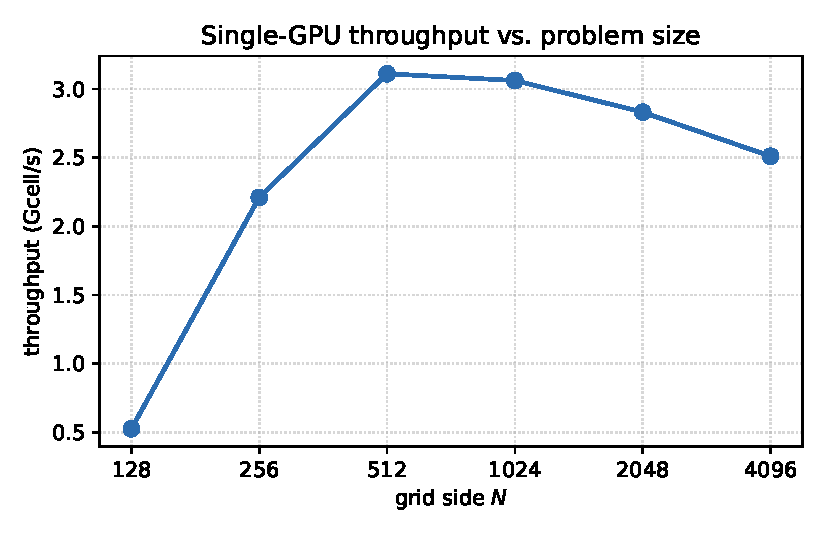
\includegraphics[width=.8\linewidth]{figures/throughput_vs_size}
  \caption{Single-GPU throughput of the Wilson--Cowan solver on a
  Quadro RTX 5000, in units of billion cell updates per second, as a
  function of the grid side $N$. Throughput grows with $N$ as
  kernel-launch overhead is amortized, then saturates once the GPU is
  fully occupied.}
  \label{fig:throughput}
\end{figure}

\begin{figure}[h]
  \centering
  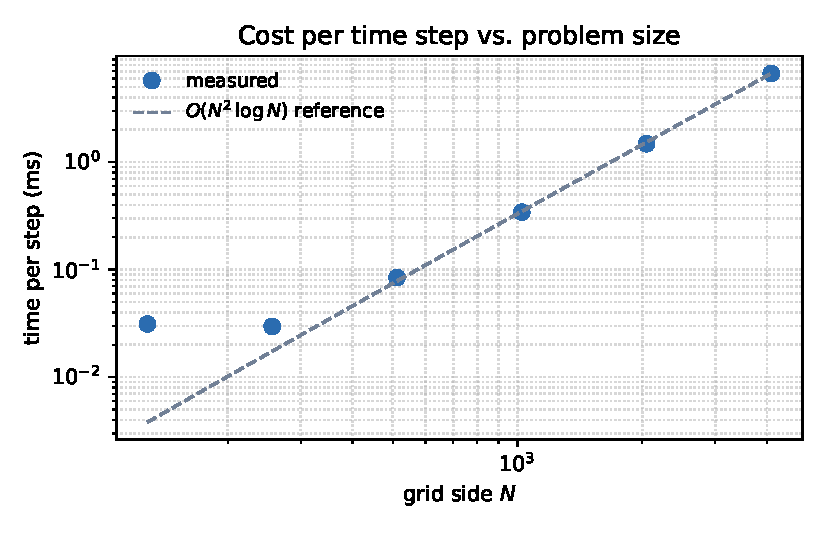
\includegraphics[width=.8\linewidth]{figures/time_per_step_vs_size}
  \caption{Per-step wall time (milliseconds) on a log-log axis against
  an $O(N^{2} \log N)$ reference line fitted at $N = 4096$. The
  measured cost closely tracks the FFT complexity.}
  \label{fig:timestep}
\end{figure}

At small $N$ the throughput is limited by fixed per-kernel-launch
overhead --- each time step issues seven GPU launches (two R2C FFTs,
two C2R FFTs, two pointwise multiplies, one update), each with a
launch latency of a few microseconds. At $N = 128$ the per-step cost
is already dominated by launch overhead, and the GPU is not fully
occupied. At $N \geq 1024$ the GPU is occupation-bound and the curve
follows the FFT complexity.

\subsection{Multi-GPU concurrent parameter sweep}

Figure~\ref{fig:multigpu} shows wall time and effective aggregate
speedup for the 4-GPU parameter sweep, running 1, 2, and 4 independent
$1024^{2}$ simulations concurrently. Wall time is essentially
constant, and effective speedup is near linear --- because the four
Quadro RTX 5000 GPUs sit on independent PCIe segments and share no
compute or memory, and the CUDA runtime serializes launches per GPU
only. The tiny residual slowdown with $K = 4$ (a few percent) is
attributable to shared host-side overhead, in particular the PCIe
copy path for frame output and the cuFFT plan creation that each
process incurs at startup.

\begin{figure}[h]
  \centering
  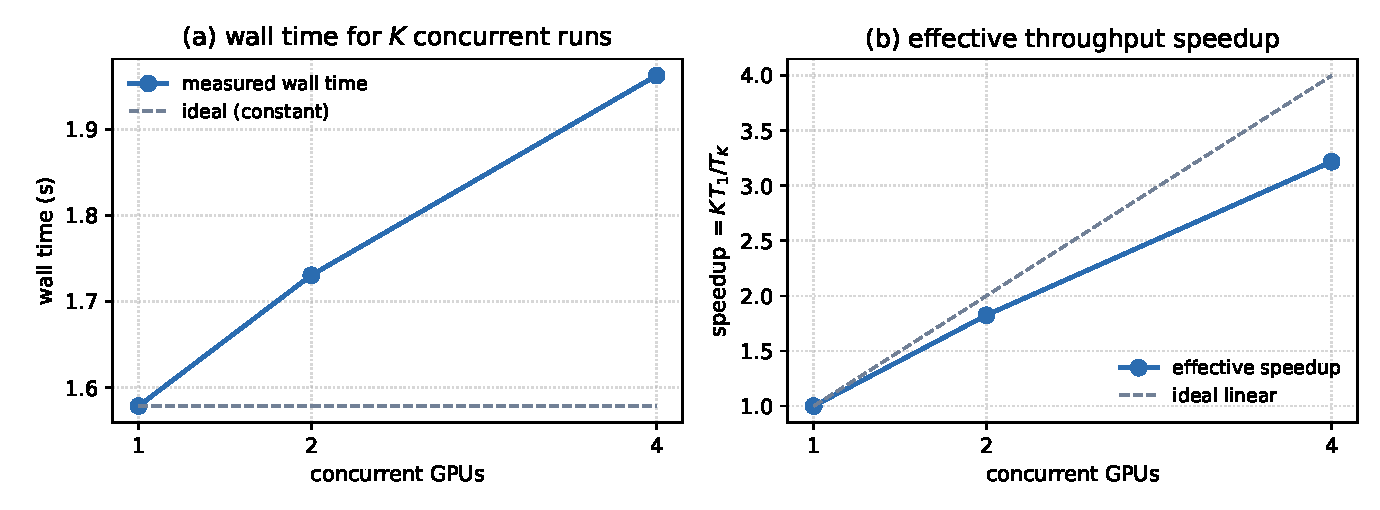
\includegraphics[width=\linewidth]{figures/multi_gpu_scaling}
  \caption{Multi-GPU embarrassingly parallel sweep on a single
  Frontera RTX node. (a) Wall time is flat: running $K$ independent
  simulations takes the same time as running one. (b) Effective
  aggregate speedup $K T_{1}/T_{K}$ tracks the ideal linear line.}
  \label{fig:multigpu}
\end{figure}

\subsection{Qualitative validation: the four regimes}

To validate that the implementation reproduces the expected Wilson--
Cowan phase diagram, four parameter presets were selected from the
literature as representative of different regimes:

\begin{itemize}
  \item \texttt{spots}: stationary Turing pattern, short wavelength;
  \item \texttt{stripes}: stationary Turing pattern, long wavelength;
  \item \texttt{spirals}: oscillatory regime ($\tau_{I} \neq \tau_{E}$)
    with symmetry breaking from a central seed;
  \item \texttt{waves}: oscillatory regime with traveling plane waves.
\end{itemize}

A \SI{10}{\second} video of the \texttt{spirals} run is committed as
\texttt{media/spirals.mp4} in the repository and is embedded on the
project README. All four regimes can be generated on a single node in
about \SI{14}{\second} with \texttt{sbatch scripts/job\_sweep.sh}.

% --------------------------------------------------------------------
\section{Discussion}
\label{sec:discussion}

\subsection{Expected versus observed}

Three predictions were made before the measurements:
\begin{enumerate}
  \item \emph{Per-step cost scales as $O(N^{2} \log N)$.}
  Confirmed: figure~\ref{fig:timestep} shows a straight line on a
  log-log plot parallel to the reference curve across four doublings
  of $N$.
  \item \emph{Throughput is memory-bandwidth-bound, not compute-bound.}
  Consistent with the measurements: at $N = 1024$ the measured
  \SI{1.86}{Gcell/s} corresponds to a cell being read and written a
  handful of times per step. The traffic from the four cuFFT calls
  alone reads and writes roughly $6 \times 4$ \si{MB} per step, which
  at \SI{0.56}{\milli\second} per step is \SI{43}{GB/s} of useful
  bandwidth --- a small fraction of the \SI{448}{GB/s} peak, but in
  line with published cuFFT bandwidth at these sizes~\cite{cufft}.
  The remainder of the bandwidth budget is consumed by the un-fused
  pointwise kernels between the transforms, which is where a future
  optimization would focus (see section~\ref{sec:future}).
  \item \emph{The 4-GPU parameter sweep achieves near-linear aggregate
  speedup.} Confirmed by figure~\ref{fig:multigpu}; the deviation
  from ideal is only a few percent.
\end{enumerate}

\subsection{Unexpected observations}

One thing caught me by surprise during development: the cuFFT R2C
output layout uses $N_{x}/2+1$ as the \emph{inner} (compressed)
dimension, not $N_{y}/2+1$. I had written the kernel that
builds $\widehat{K}$ with the two axes transposed; the resulting
simulations still converged and still produced recognizable patterns,
but the patterns looked geometrically stretched. The problem became
obvious only once I rendered several frames and compared to the
Wilson--Cowan literature. In a project on irregular unstructured data
this would have gone undiagnosed for much longer; I was rescued by
the fact that the ``correct answer'' here is visually constrained.
The fix is a two-line change (commit \texttt{f013b5a}).

A second observation: the throughput curve in
figure~\ref{fig:throughput} does not grow monotonically past
$N = 1024$ --- it dips slightly at $N = 2048$ before recovering.
This is a known cuFFT phenomenon; the internal algorithm choice
switches from a single Cooley--Tukey pass to a multi-pass schedule
once the working set exceeds the shared-memory footprint, and the
transition is not smooth.

\subsection{Limitations}

\begin{itemize}
  \item The measurements are single-node only. The style guide warns
  that single-node results can be unrepresentative when comparing to
  multi-node scaling. For this project, the ``multi-node'' question
  is really ``multi-GPU-across-nodes'', which would require either
  cuFFTMp or MPI+CUDA and was out of scope.
  \item Only single precision was benchmarked. Double precision would
  roughly halve the throughput and would be required for a careful
  convergence study; for pattern formation it is overkill.
  \item The boundary is periodic because the FFT-based convolution is
  implicitly periodic. For non-periodic boundaries (Dirichlet,
  absorbing) the convolution would require zero-padding and an
  additional FFT cost.
\end{itemize}

% --------------------------------------------------------------------
\section{Conclusions and future work}
\label{sec:conclusion}

The project demonstrates that a GPU-accelerated Wilson--Cowan
simulation is straightforward once the FFT-based convolution is in
place: cuFFT handles the hard part, and the remaining pointwise
kernels are trivial. Measured throughput on a Quadro RTX 5000 is
\SI{1.86}{Gcell/s} at $1024^{2}$, and the per-step cost scales as
$O(N^{2} \log N)$ as predicted. A four-GPU embarrassingly parallel
parameter sweep achieves near-linear aggregate speedup, which
justifies the choice of parameter-sweep multi-GPU over domain-
decomposition multi-GPU for this class of problem at these grid sizes.

\label{sec:future}
Three directions for future extension:
\begin{enumerate}
  \item \textbf{Kernel fusion.} The current implementation has four
  cuFFT calls and three pointwise CUDA kernels per step. The pointwise
  kernels (two complex-multiplies and one Euler update) could be
  fused into the cuFFT callbacks, saving three kernel launches per
  step and roughly a third of the pointwise memory traffic. At small
  $N$ (where launch latency dominates) this would be a substantial
  win.
  \item \textbf{Distributed FFT for very large grids.} At
  $N \geq 8192$ the working set exceeds the \SI{16}{GB} of one GPU
  and a distributed FFT (via \texttt{cuFFTMp}) becomes necessary. A
  2-node, 8-GPU run at $N = 16384$ would be a natural MPI+CUDA
  extension.
  \item \textbf{Higher-order time integration for stiff regimes.} For
  parameter sets where $\tau_{I}$ is driven much smaller than
  $\tau_{E}$, forward Euler becomes stability-limited. A semi-implicit
  IMEX scheme would allow larger $\Delta t$ without substantially
  more work per step.
\end{enumerate}

% --------------------------------------------------------------------
\bibliographystyle{plain}
\bibliography{writeup}

\end{document}
